\label{sec:theory-sm}
\subsection{Overview: Particles and Interactions in Standard Model}

The Standard Model has two types of particles: Bosons and Fermions; the former have integer spins and the later have fractional spins. All particles in the Standard Model are summarized in Fig. \ref{fig:theory-sm}.

The fermions include leptons and quarks, and are what we normally know as matter. They have spin $\frac{1}{2}$. Electrons($e^-$), muons($\mu^-$), taus($\tau^{-}$) and their anti-particles ($e^+,\mu^+,\tau^+$) are leptons which carry electric charges. Associated with these charged leptons are the neutral neutrinos ($\nu_e,\nu_{\mu},\nu_{\tau}$) and their anti-particles ($\bar{\nu_e},\bar{\nu_{\mu}},\bar{\nu_{\tau}}$). There are three ``up'' type quarks with $\frac{2}{3}$ electric charges ($u$, $c$, $t$) and three ``down'' type quarks with $-\frac{1}{3}$ electric charges. 

The spin 1 bosons are the mediators of fundamental interactions. In total, there are four types of interactions namely: strong, weak, electromagnetic(EM) and gravitational. Within the Standard Model framework, since gravity is much weaker than the others, we only consider the first three kinds of forces. At subatomic scale, the strong force has the greatest strength and EM force is the second in the rank. Among the force carriers photon($\gamma$) and gluon($g$) are massless particles and mediate the electromagnetic and strong interactions respectively. The $W^{\pm}$ and $Z$ bosons are massive particles and carry the weak force. 

All fermions interact through week forces. Only electrically charged fermions interact with the photon(EM force). Only the quarks carry color(the strong interaction version of electric charge) and interact with gluons. The Higgs boson is the only spin 0 boson within the SM and generates mass for $W^{\pm}/Z$ bosons and fermions (except neutrinos). The mechanism of mass generation is covered later in this chapter. The Higgs boson also couples to itself. 

\begin{figure}[htpb!]
\begin{center}
  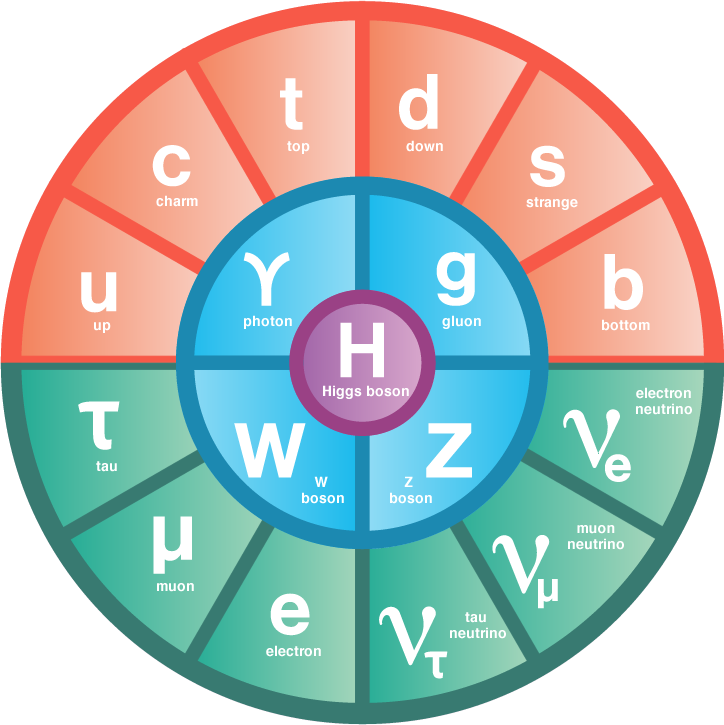
\includegraphics[width=0.45\linewidth]{figures/theory/SM}
\caption{Fundamental particles within the Standard Model}
\label{fig:theory-sm}
\end{center}
\end{figure}

\subsection{Standard Model in QFT Form}

Quantum Field Theory (QFT) the marriage between Quantum Mechanics and Special Relativity, is the modern formalism to describe fundamental physics. In the language of QFT, fields of creation and annihilation operators allow us to calculate the probability distributions of particles which are excited states of fields over time and space. The Standard Model is a special gauge QFT which is invariant with respect to the internal (gauge) $SU(3)\times SU(2)\times U(1)$ symmetry. The gauge symmetries, which give birth to the gauge bosons, are field local symmetries in addition to the global symmetries such as spatial and time. 

The Lagrangian which governs the motion of SM particles can be separated into two parts: $SU(3)$ and $SU(2)\times U(1)$. The $SU(3)$ part of the Lagrangian corresponding to the strong interaction goes as in Eq.\ref{eq:l-su3}. The first term has $F^{a}_{\mu\nu}  = \partial_{\mu}G^a_{\nu}-\partial_{\nu}G^a_{\mu}+g_3f^{abc}G^b_{\mu}G^c_{\nu}$, where $G$ is the gauge field (in this case gluons), $f^{abc}$ is the structure constant of $SU(3)$ group and $g_3$ is the coupling strength for strong interaction. The second term has $\slashed{D} = \gamma^{\mu}(\partial_{\mu}- i\frac{g_3}{2}\lambda^aG^a_{\mu})$, where $\gamma$'s are the Dirac matrices, the $\lambda$'s are the $SU(3)$ matrices and $\psi$ are the quark fields. 
\begin{equation}
  \mathcal{L}_{SU(3)} = -\frac{1}{4}F^{a}_{\mu\nu}F_{a}^{\mu\nu}+ \bar{\psi}(i\slashed{D}) \psi
  \label{eq:l-su3}
\end{equation}

The $SU(2)\times U(1)$ part of the Lagrangian is the unified theory which combines electromagnetic and weak forces. Both kinds of forces exhibit similar properties in the energy scale of \GeV and can be regarded as the same kind of force. This part of the Lagrangian has the same terms as in Eq.\ref{eq:l-su3}, replacing the gauge/fermion fields, structure constants, coupling strength and group matrices to be the corresponding ones in $SU(2)$ and $U(1)$. Note that $U(1)$ group is Abelian and hence $f^{abc}=0$ and the group matrix is a number, while for $SU(2)$ the group matrices are the Pauli matrices ($\sigma$). 
